\addcontentsline{toc}{chapter}{Занятие 15. Характеристические функции}
\chapter*{Занятие 15. Характеристические функции}

\addcontentsline{toc}{section}{Контрольные вопросы и задания}
\section*{Контрольные вопросы и задания}

\subsubsection*{Приведите определение характеристической функции случайной величины, сформулируйте свойства характеристической функции; запишите характеристические функции основных вероятностных распределений.}

Характеристической функцией случайной величины $ \xi $ называется функция $ \varphi_{ \xi } \left( t \right) = Me^{it \xi } = M \cos t \xi + iM \sin t \xi $, где $i$ ---
это мнимая единица, $t \in \mathbb{R}$.

В терминах функции распределения
$$ \varphi_{ \xi } \left( t \right) =
\int \limits_{- \infty }^{+ \infty } e^{itx} dF_{ \xi } \left( x \right).$$

В терминах плотности
$$ \varphi_{ \xi } \left( t \right) =
\int \limits_{- \infty }^{+ \infty } e^{itx} p \left( x \right) dx$$
--- преобразование Фурье для плотности.

Свойства:
\begin{enumerate}
\item $ \left| \varphi_{ \xi } \left( t \right) \right| \leq 1$ и $ \varphi_{ \xi } \left( 0 \right) = 1$;
\item $ \varphi_{ \xi } \left( t \right) = \overline{ \varphi_{ \xi } \left( -t \right)}$, имеется в виду комплексно сопряжённое;
\item $ \varphi_{ \xi }$ равномерно непрерывна на числовой оси $ \mathbb{R}$.
Это означает,
что
$$ \forall \epsilon > 0 \,
\exists \delta > 0: \,
\left| t_1 - t_2 \right| \leq \delta \Rightarrow \left| \varphi_{ \xi } \left( t_1 \right) - \varphi_{ \xi } \left( t_2 \right) \right| < \epsilon;$$
\item $ \varphi_{ \xi }$ --- неотрицательно определённая:
$$ \forall t_1, \dotsc, t_n \in \mathbb{R}, \,
\lambda_1, \dotsc, \lambda_n \in \mathbb{R}: \,
\sum \limits_{k,j=1}^n \varphi_{ \xi } \left( t_k - t_j \right) \lambda_k \lambda_j \geq 0.$$
\end{enumerate}

Примеры характеристических функций на известных распределениях:
\begin{enumerate}
\item биномиальное: $ \xi = 0, \dotsc, n$, есть параметр $p \in \left( 0, 1 \right) $, а вероятность $P \left\{ \xi = k \right\} = C_n^k p^k \left( 1 - p \right)^{n-k}$.
Тогда
$$ \varphi_{ \xi } \left( t \right) =
\left[ \left( e^{it} - 1 \right) p + 1 \right]^n;$$
\item геометрическое: $ \xi = 0, 1, 2, \dotsc $, есть число $p \in \left( 0, 1 \right) $.
Тогда
$$P \left( \xi = k \right) = \left( 1-p \right) p^k, \,
\varphi_{ \xi } \left( t \right) = Me^{it \xi } = \sum \limits_{k=0}^{ \infty } \left( 1-p \right) p^k \left( e^{it} \right)^k = \frac{1-p}{1-pe^{it}};$$
\item пуассоновское с параметром $ \lambda > 0$.
Здесь
$$ \xi = 0, 1, \dotsc, \,
P \left\{ \xi = k \right\} = e^{- \lambda } \cdot \frac{ \lambda^k}{k!}.$$
Так что
$$ \varphi_{ \xi } \left( t \right) =
\sum \limits_{k=0}^{ \infty } e^{- \lambda } \cdot \frac{ \lambda^k \left( e^{it} \right)^k}{k!} =
e^{ \lambda \left( e^{it} - 1 \right) };$$
\item равномерное.
Пусть $ \xi $ имеет плотность
$$ \mathbbm{1}_{ \left[ a, b \right] } \left( x \right) \cdot \frac{1}{b-a}.$$
Тогда
$$ \varphi_{ \xi } \left( t \right) =
\frac{1}{b-a} \int \limits_a^b e^{itx} dx =
\left( e^{itb} - e^{ita} \right) \cdot \frac{1}{it \left( b-a \right)};$$
\item показательное распределение с параметром $ \lambda > 0$.
Здесь плотность имеет вид $p \left( x \right) = \mathbbm{1}_{ \left[ 0, + \infty \right) } \left( x \right) \lambda e^{- \lambda x}$.
Поэтому
$$ \varphi_{ \xi } \left( t \right) =
\int \limits_0^{+ \infty } \lambda e^{- \left( \lambda - it \right) x} dx =
\frac{ \lambda }{ \lambda - it};$$
\item гауссовское.
Возьмём вначале $N \left( 0, 1 \right) $.
Это
$$p \left( x \right) =
\frac{1}{ \sqrt{2 \pi }} \cdot e^{- \frac{x^2}{2}}.$$
Получим $ \varphi_{ \xi } \left( t \right) = e^{- \frac{t^2}{2}}$.
В общем виде $ \varphi \left( t \right) = Me^{it \left( a + \sqrt{ \sigma^2} \xi \right) } = e^{ita} e^{- \frac{t^2 \sigma^2}{2}}$;
\item $ \varphi \left( t \right) = e^{- \left| t \right| }$ --- характеристическая функция для распределения Коши.
\end{enumerate}

\subsubsection*{Сформулируйте теорему Бохнера, теорему Пойя.}

Теорема Бохнера-Хинчина.
Функция $ \varphi: \mathbb{R} \rightarrow \mathbb{C}$ является характеристической функцией некоторого вероятностного распределения (т.е. некоторой случайной величины)
тогда и только тогда, когда $ \phi $ обладает свойствами 1) --- 4).
Условие 3) можно заменить просто непрерывностью.

Теорема Пойа.
Пусть функция $ \varphi: \mathbb{R} \rightarrow \mathbb{R}$ --- чётная, непрерывная,
выпуклая вниз на $ \left[ 0, + \infty \right), \, \varphi \left( 0 \right) = 1, \, \varphi $ убывает у нулю на $+ \infty $.
Тогда $ \varphi $ --- характеристическая.

\subsubsection*{Запишите формулу обращения для характеристических функций.}

Теорема (формула восстановления для характеристических функций).
Пусть $ a < b$ --- точки непрерывности функции распределения $F$.
Тогда
$$F \left( b \right) - F \left( a \right) =
\lim \limits_{c \to + \infty } \frac{1}{2 \pi } \int \limits_{-c}^c \frac{e^{-ita} - e^{-itb}}{it} \cdot \varphi(t) dt.$$

\subsubsection*{Какая связь между производными характеристической функции и моментами случайной величины?}

Лемма.
Пусть $M \left| \xi \right|^n < + \infty $, тогда $ \exists \varphi^{ \left( k \right) } \left( 0 \right) $ для
$k = 1, \dotsc, n$ и
$$M \xi^k =
\left( -i \right)^k \varphi^{ \left( k \right) } \left( 0 \right).$$

Лемма.
Пусть $ \exists \varphi^{ \left( 2n \right) } \left( 0 \right) $.
Тогда $M \xi^{2n} < + \infty $ и
$$M \xi^k = \left( -i \right)^k \varphi^{ \left( k \right) } \left( 0 \right) \,
\forall k = 1, \dotsc, 2n.$$

\addcontentsline{toc}{section}{Аудиторные задачи}
\section*{Аудиторные задачи}

\subsubsection*{15.3}

\textit{Задание.} Случайная величина $ \xi $ принимает значения $1$ и $- 1$ с вероятностью $1 / 2$ каждое.
Найдите характеристическую функцию $ \xi $.

\textit{Решение.} $ \xi $ --- случайная величина.
$$P \left( \xi = 1 \right) =
P \left( \xi = - 1 \right) =
\frac{1}{2}.$$
По определению
$$ \varphi_{ \xi } \left( t \right) =
Me^{it \xi } =
e^{it} \cdot \frac{1}{2} + e^{- it} \cdot \frac{1}{2} =
\frac{1}{2} \left( e^{it} + e^{- it} \right) =
\cos t.$$

\subsubsection*{15.4}

\textit{Задание.} Случайная величина $ \xi $ имеет плотность распределения
$$p \left( x \right) =
\begin{cases}
0, \qquad \left| x \right| > a, \\
\frac{1}{a} \left( 1 - \frac{ \left| x \right| }{a} \right), \qquad \left| x \right| \geq a.
\end{cases}$$
Докажите, что её характеристическая функция
$$ \varphi \left( t \right) =
\begin{cases}
1 - \left| t \right|, \qquad \left| t \right| \leq 1, \\
0, \qquad \left| t \right| > 1.
\end{cases}$$

\textit{Решение.} $ \xi $ --- случайная величина.
Её плотность распределения ---
$$p \left( x \right) =
\begin{cases}
0, \qquad \left| x \right| > a, \\
\frac{1}{a} \left( 1 - \frac{ \left| x \right| }{a} \right), \qquad \left| x \right| \geq a.
\end{cases}$$
По определению
$$ \varphi_{ \xi } \left( t \right) =
\int \limits_{- a}^a e^{itx} \cdot \frac{1}{a} \left( 1 - \frac{ \left| x \right| }{a} \right) dx.$$
Действительная часть подынтегральной функции чётная
$$ \varphi_{ \xi } \left( t \right) =
2 \cdot \frac{1}{a} \int \limits_0^a \cos \left( tx \right) \left( 1 - \frac{x}{a} \right) dx.$$
Раскроем скобки и возьмём второй интеграл по частям
$$ \varphi_{ \xi } \left( t \right) =
\left. 2 \cdot \frac{1}{a} \cdot \frac{ \sin \left( tx \right) }{t} \right|_0^a -
\frac{2}{a} \left( \left. \frac{x \sin \left( tx \right) }{t} \right|_0^a - \int \limits_0^a \frac{ \sin \left( tx \right) }{t} dx \right).$$
Подставим пределы интегрирования и возьмём интеграл
$$ \varphi_{ \xi } \left( t \right) =
\frac{2}{a} \cdot \frac{ \sin \left( at \right) }{t} - \frac{2}{a} \cdot \frac{ \sin \left( at \right) }{t} - \frac{ \cos \left( at \right) - 1}{t^2} \cdot \frac{2}{a^2}.$$
Первые 2 слагаемых уничтожаются
$$ \varphi_{ \xi } \left( t \right) =
\frac{2}{a^2} \cdot \frac{1 - \cos \left( at \right) }{t^2}.$$

\subsubsection*{15.5}

\textit{Задание.} Найдите закон распределения, которому соответствует характеристическая функция
$$ \begin{cases}
1 - \left| t \right|, \qquad \left| t \right| \leq 1, \\
0, \qquad \left| t \right| > 1.
\end{cases}$$

\textit{Решение.}
$$ \int \limits_{- \infty }^{+ \infty } \left| \varphi \left( t \right) \right| dt =
\int \limits_{- 1}^1 \left| 1 - \left| t \right| \right| dt.$$
При изменении $t$ на $ \left( - t \right) $ ничего не изменится, значит подынтегральная функция чётная
$$ \int \limits_{- \infty }^{+ \infty } \left| \varphi \left( t \right) \right| dt =
2 \int \limits_0^1 \left( 1 - t \right) dt =
2 \left. \left( t - \frac{t^2}{2} \right) \right|_0^1 =
2 \left( 1 - \frac{1}{2} \right) =
2 \cdot \frac{1}{2} =
1 < + \infty.$$
Отсюда следует, что функция абсолютно интегрируема.

$$p \left( t \right) =
\frac{1}{2 \pi } \int \limits_{-1}^1 e^{- itx} \left( 1 - \left| t \right| \right) dt =
2 \cdot \frac{1}{2 \pi } \int \limits_0^1 \cos \left( tx \right) \left( 1 - t \right) dt.$$
Интегрируем частями
$$p \left( t \right) =
\frac{1}{ \pi } \int \limits_0^1 \cos \left( tx \right) dt - \frac{1}{ \pi } \int \limits_0^1 t \cos \left( tx \right) dt =
\frac{1}{ \pi } \left( \frac{ \sin x}{x} - \frac{ \sin x}{x} + \frac{1 - \cos x}{x^2} \right).$$
Первые 2 слагаемых уничтожаются
$$p \left( t \right) =
\frac{1 - \cos x}{ \pi x^2}.$$

\subsubsection*{15.6}

\textit{Задание.} Докажите, что следующие функции являются характеристическими:
\begin{enumerate}[label=\alph*)]
\item $ \cos^2 t$;
\item $e^{- t^2}$;
\item $e^{- \left| t \right| }$.
\end{enumerate}

\textit{Решение.}
\begin{enumerate}[label=\alph*)]
\item Нарисуем график (рис. \ref{fig:1562}).

\begin{figure}[h!]
  \centering
  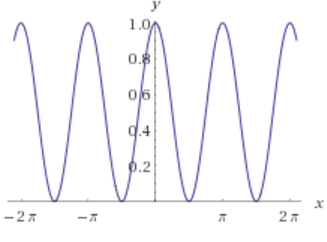
\includegraphics[width=.4\textwidth]{./pictures/15_6_2.png}
  \caption{График функции $ \cos^2 t$}
  \label{fig:1562}
\end{figure}

Теорема Пойа не подходит, но $ \cos t$ является характеристической функцией.
Пусть $ \xi_1, \dotsc, \xi_n$ --- независимые случайные величины.
Тогда
$$ \varphi_{ \xi_1 + \xi_2 + \dotsc + \xi_n} \left( t \right) =
\varphi_{ \xi_1} \left( t \right) \cdot \varphi_{ \xi_2} \left( t \right) \cdot \dotsc \cdot \varphi_{ \xi_n} \left( t \right).$$

Пусть $ \xi_2, \, \xi_2$ --- независимые случайные величины с распределением
$$P \left( \xi_1 = 1 \right) =
P \left( \xi_2 = - 1 \right) =
\frac{1}{2}.$$
Тогда характеристическая функция их суммы $ \varphi_{ \xi_1 + \xi_2} \left( t \right) = \varphi_{ \xi_1} \left( t \right) \cdot \varphi_{ \xi_2} \left( t \right) $.
Из задачи 15.3 $ \varphi_{ \xi_1 + \xi_2} \left( t \right) = \cos^2 t$.
Предъявили ту случайную величину, для которой это является характеристической функцией.

\item нарисуем график функции (рис. \ref{fig:1561}).

\begin{figure}[h!]
  \centering
  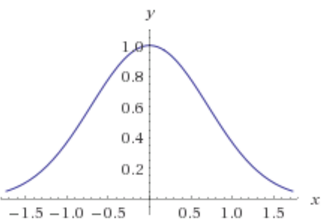
\includegraphics[width=.4\textwidth]{./pictures/15_6_1.png}
  \caption{График функции $e^{- t^2}$}
  \label{fig:1561}
\end{figure}

Это характеристическая функция случайной величины $ \xi \sim N \left( 0, 2 \right) $;

\item используем теорему Пойа.
Нарисуем график (рис. \ref{fig:156}).

\begin{figure}[h!]
  \centering
  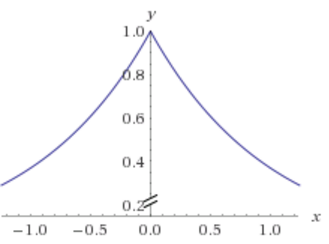
\includegraphics[width=.4\textwidth]{./pictures/15_6.png}
  \caption{График функции $e^{ - \left| t \right| }$}
  \label{fig:156}
\end{figure}

В нуле --- единица, функция чётная, неотрицательная, выпуклая вниз, стремится к нулю.
По теореме Пойа эта функция является характеристической.
\end{enumerate}

\subsubsection*{15.7}

\textit{Задание.} Докажите, что следующие функции не могут быть характеристическими:
\begin{enumerate}[label=\alph*)]
\item $e^{- i \left| t \right| }$;
\item $ \cos t^2$.
\end{enumerate}

\textit{Решение.}
\begin{enumerate}[label=\alph*)]
\item $e^{- i \left| t \right| } = \varphi \left( t \right)$.

Проверим сопряжённость.

$$e^{- i \left| t \right| \neq e^{i \left| - t \right| }}.$$
Отсюда следует, что нарушается условие комплексной сопряжённости;
\item схематически нарисуем график этой функции (рис. \ref{fig:157}).

\begin{figure}[h!]
  \centering
  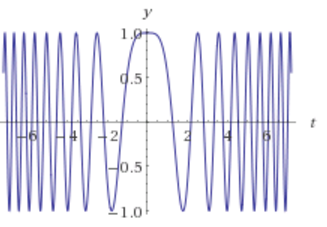
\includegraphics[width=.4\textwidth]{./pictures/15_7.png}
  \caption{График функции $ \cos t^2$}
  \label{fig:157}
\end{figure}

Нарушается равномерная непрерывность.

Покажем это.

Покажем, что размах --- 2.
Берём $t_1 = \sqrt{2k \pi }$, а $t_2 = \sqrt{2k \pi + \pi }$.
Смотрим на их разность
$$ \left| t_2 - t_1 \right| =
\frac{ \pi }{ \sqrt{2k \pi } + \sqrt{2k \pi + \pi }}.$$

Когда $k \rightarrow \infty $, то $ \left| t_2 - t_1 \right| \rightarrow 0$.
Значит можем найти как угодно близкие точки.
Смотрим на разность значений функций в этих точках $ \left| \varphi \left( t_2 \right) - \varphi \left( t_1 \right) \right| = \left| 1 - \left( -1 \right) \right| = 2$.

Расстояние равно двум, остаётся постоянным, к нулю не стремится.
\end{enumerate}

\subsubsection*{15.8}

\textit{Задание.}
Докажите, что если $ \varphi \left( t \right) $ является характеристической функцией, то $ \left| \varphi \left( t \right) \right|^2$ тоже есть характеристической функцией.

\textit{Решение.} $ \left| \varphi \left( t \right) \right|^2 = \varphi \left( t \right) \overline{ \varphi \left( t \right) }$.
По одному из свойств это равно $ \varphi \left( t \right) \varphi \left( - t \right) $.

По определению характеристической функции $ \varphi \left( t \right) = Me^{it \xi }$.

Тогда $ \varphi \left( - t \right) = Me^{- it \xi } = Me^{it \left( - \xi \right) } = \varphi_{- \xi } \left( t \right) $.

Пусть $ \xi_1, \, \xi_2$ ---
независимые случайные величины с характеристической функцией $ \varphi \left( t \right) = \varphi_{ \xi_1} \left( t \right) = \varphi_{ \xi_2} \left( t \right) $.

Тогда
$ \varphi_{ \xi_1 - \xi_2} \left( t \right) =
\varphi_{ \xi_1} \left( t \right) \varphi_{- \xi} \left( t \right) =
\varphi_{ \xi_1} \left( t \right) \varphi_{ \xi_2} \left( - t \right) $.
Это одна и та же характеристическая функция, потому это равно $ \varphi \left( t \right) \varphi \left( - t \right) $.
